\aufgabe{Categorical ALE}{

In this exercise, we use the German Credit dataset (\textit{datasets/credit.csv}) and a random forest 
to predict whether a customer is a high or low risk for a bank. 
The dataset could be found in \textit{credit.csv}. 
The following table gives an overview: 

\begin{table}[ht]
\centering
\begin{tabular}{rllrr}
  \hline
 & name & type & mean & nlevs \\ 
  \hline
1 & credit\_risk & factor &  &   2 \\ 
  2 & age & integer & 35.55 &   0 \\ 
  3 & amount & integer & 3271.26 &   0 \\ 
  4 & credit\_history & factor &  &   5 \\ 
  5 & duration & integer & 20.90 &   0 \\ 
  6 & employment\_duration & factor &  &   5 \\ 
  7 & personal\_status\_sex & factor &  &   4 \\ 
  8 & purpose & factor &  &  10 \\ 
   \hline
\end{tabular}
\end{table}

Since the decision of whether a person gets a loan can have serious implications
on the person's life, banks are subordinate to regulations and must disclose 
the underlying mechanism of their used model to authorities. 
Since looking on the single trees is not feasible to uncover the internals of a random forest,
(model-agnostic) interpretation methods should help to unfold the underlying mechanisms
and to explain specific decisions. 

\begin{enumerate}[a)]
\item 
Since the regulations require that the model does not discriminate against 
certain demographic groups, you want to evaluate the feature effect of
\texttt{personal\_status\_sex} of the fitted forest model. 
Your colleague provides Figure~\ref{fig:pdp}. Interprete the PDP.

\begin{figure}[!ht]
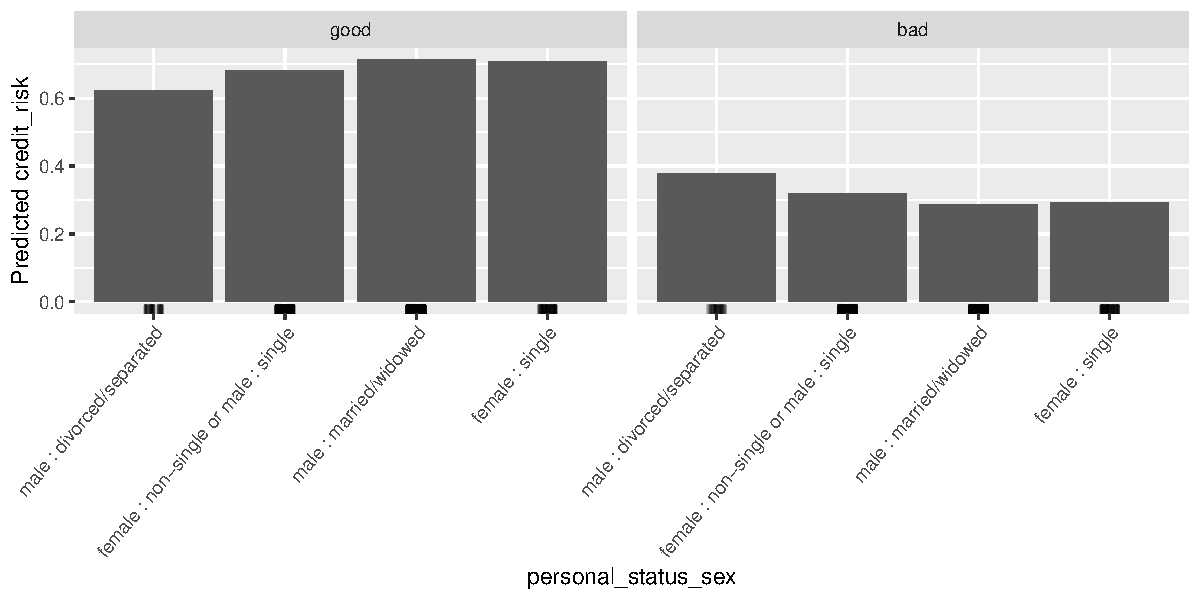
\includegraphics[width=\maxwidth,]{figure/PDP_Personal_Status_Sex.pdf}
\caption{PDP of personal\_Status\_sex}
\label{fig:pdp}
\end{figure}

\item You also request an ALE plot from your colleague. 
Give reasons why and in which situations inspecting ALE plots besides PDPs is advisable?

\item 
Because the ALE models accumulates effects in a specific direction, the feature values must have an order by definition. However, there is no natural order to categorical/nominal features like \texttt{personal\_status\_sex}. 
In order to derive an artificial order, Molnar 2022 (Chapter 8.2)\footnote{https://christophm.github.io/interpretable-ml-book/ale.html} proposes to order the categories of the features $x_s$ according to their similarity based on other/remaining features $x_c \in X_C$. 
Read the corresponding subsection in Molnar 2022.

In detail, the approach has the following steps: 

\begin{enumerate}[1)]
  \item For each feature $x_c \in X_C$ do the following: 
  \begin{enumerate}
    \item Get the conditional empirical distributions of $x_c$ given the categories of $x_s$: \\
     For numeric feature $x_c$, estimate the cumulative distribution function for each category of $x_s$ separately and derive its values at predefined points (e.g., at deciles of $x_c$). 
     For categorical feature $x_c$ derive the relative frequency tables for each category of $x_s$ separately.
    \item Compute the pairwise distances of distributions for each pair of categories of $x_s$:\\ 
    For numeric feature $x_c$, the distance is equal to the absolute maximum point-wise distance of the two empirical distribution functions. For categorical feature $x_c$, the distance is equal to the sum of the absolute difference of both relative frequency tables.   
  \end{enumerate}
  \item end for
  \item Sum up the pairwise distances of the distributions over features $x_c$ in $X_C$ for each class pair of $x_s$. 
  \item Reduce the resulting distance matrix to a single dimension using multi-dimensional scaling.
  \item Order the categories of $x_s$ according to the obtained similarity values.
\end{enumerate}

Your colleague already implemented some parts of the algorithm. Depending on your 
preference, you can access either the R code in \textit{catale.R} or the 
Python code in \textit{catale.py}.
Your colleague needs your help with implementing the computation of the distance of 
distribution for a \textbf{categorical} feature $x_c$ in 
\texttt{get\_diff\_cat()}. 

\begin{itemize}
  \item Have a look on the function \texttt{order\_levels()} and \texttt{get\_diff\_numeric()}. 
  Locate the steps of above's  algorithmic description in the underlying code.
  At the end of the script examples are given to run the code. 
  \item Implement the missing rows in \texttt{get\_diff\_cat()}.
  \textit{Hint:} The command \texttt{expand.grid(levels(feature.j), levels(feature.j))} creates the first two columns in 
your resulting dataset - the pairwise class combinations for $x_s$.
  \item Test your function with the provided example code (end of script). 
  Your returned \texttt{data.frame} for \texttt{personal\_status\_sex} as $x_s$ 
  and \texttt{employment\_duration} as $x_c$, should look 
  similar to this: 

\begin{table}[ht]
\centering
\begin{tabular}{llr}
  \hline
 class1 & class2 & dist \\ 
  \hline
male : married/widowed & male : married/widowed & 0.00 \\ 
female : non-single or male : single & male : married/widowed & 0.22 \\ 
male : divorced/separated & male : married/widowed & 0.19 \\ 
  ... & ... & ... \\
   \hline
\end{tabular}
\end{table}

\item How did your function order the levels of \texttt{personal\_status\_sex}? 
Does this order make sense to you? 

\item \textbf{Bonus:} Critically assess whether PDP/ALE alone replace a complete fairness audit.

\end{itemize}
\end{enumerate}
}